\chapter{Evaluation}
\label{cha:ergebnisse}

The robot is put into specifically designed scenarios that should trigger behavior responses from the behavior tree component. The scenario testing is done to evaluate the efficacy of the implemented behaviors in relation to the functional requirements listed in chapter 3.2.

The scenarios are executed in a simulated apartment environment as seen in figure \ref{fig:house_gazebo} and a simulated world with small round obstacles in an enclosed space as depicted in figure \ref{fig:world_gazebo}. 
\begin{center}
\begin{figure}[ht]
	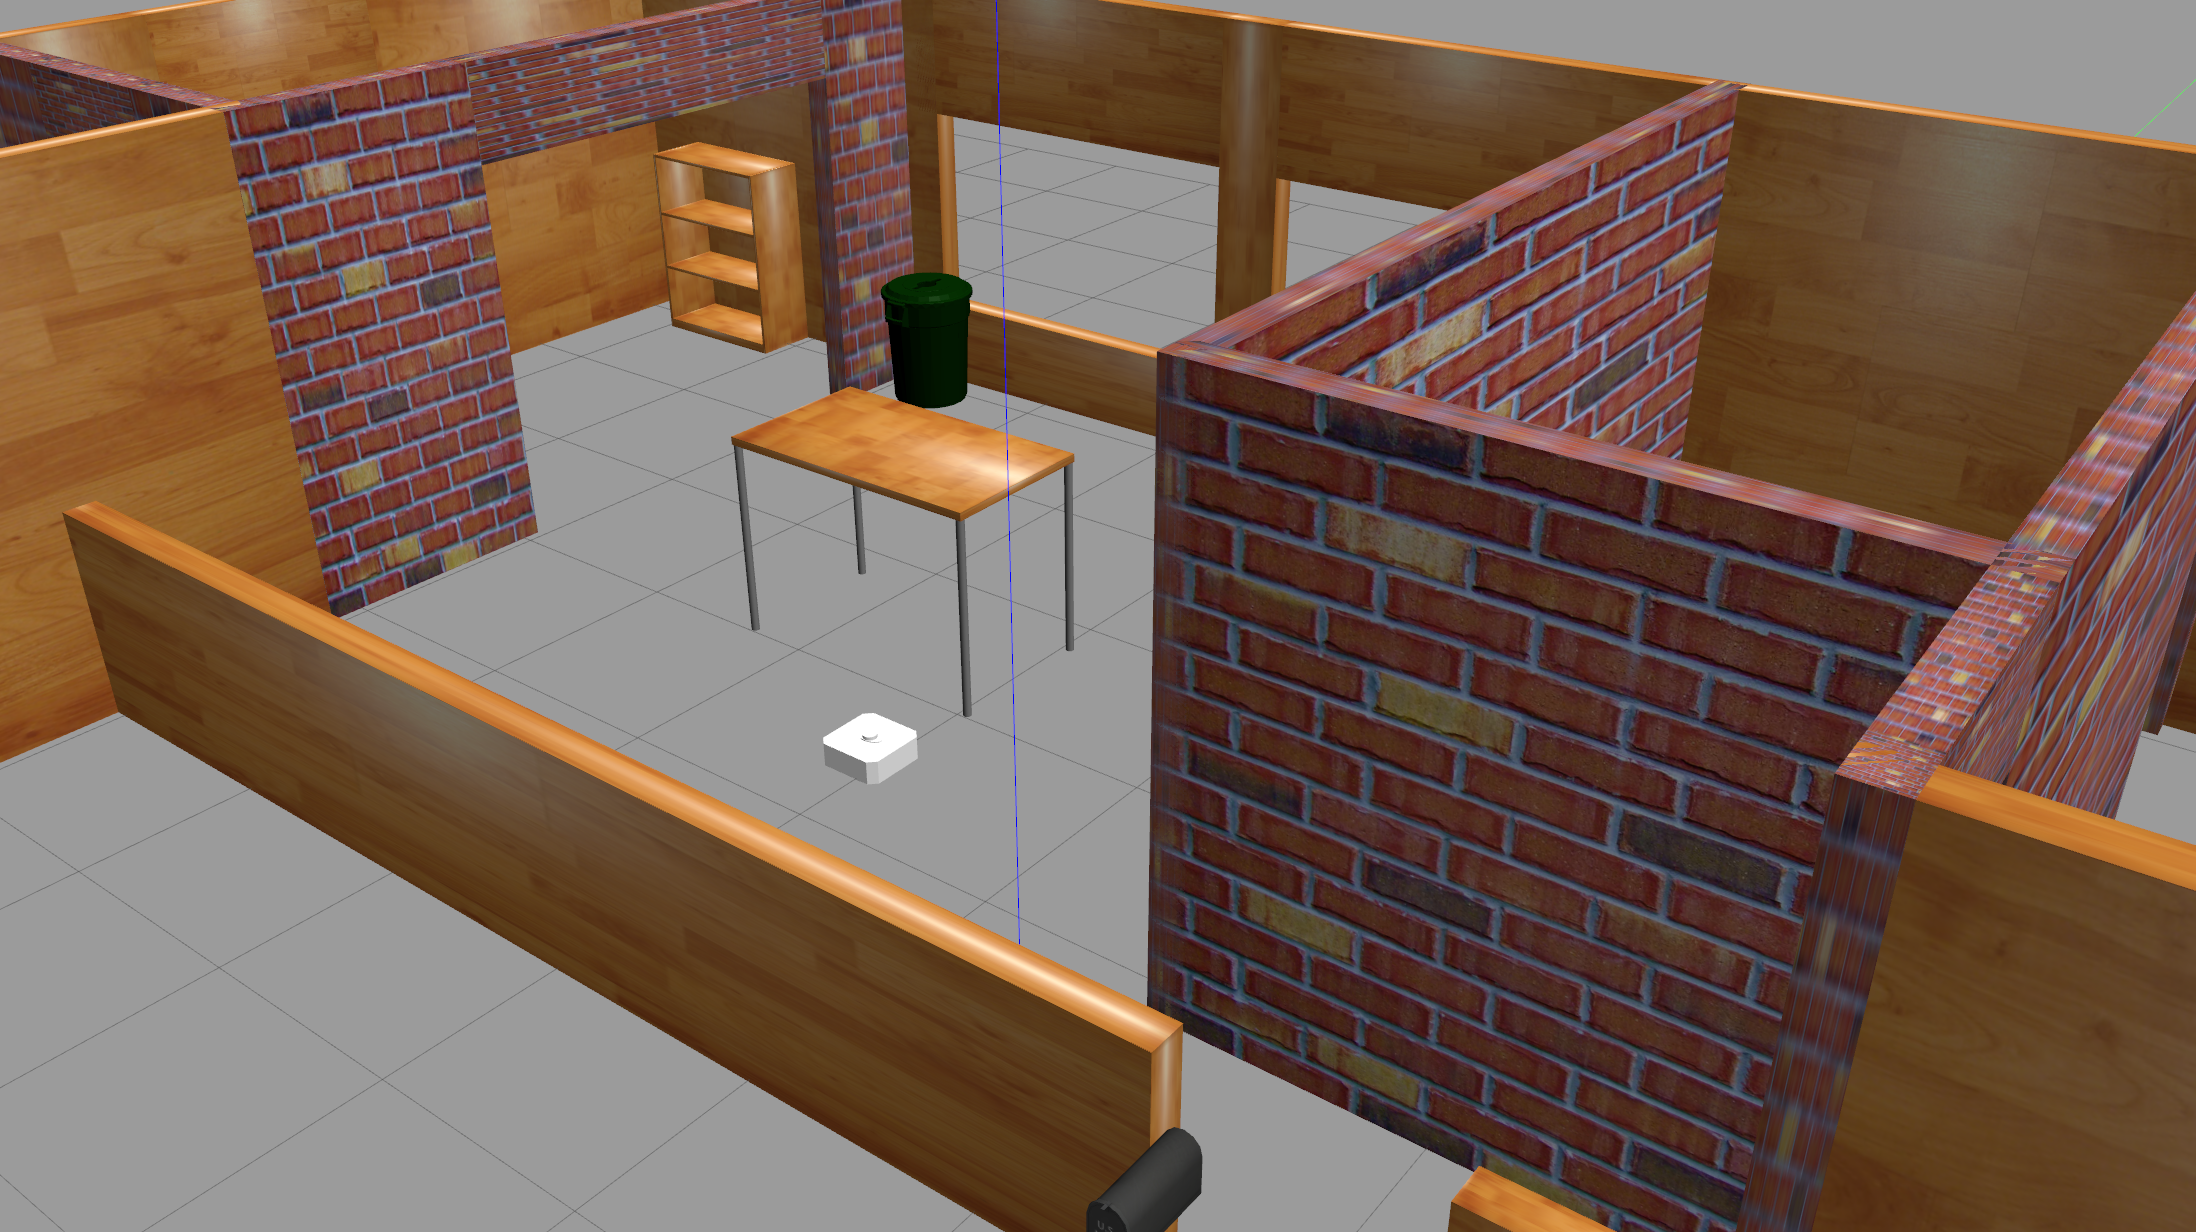
\includegraphics[width=0.75\textwidth]{images/house_env.png}
	\caption{Apartment Environment in Gazebo}
	\label{fig:house_gazebo}
\end{figure}
\end{center}

\begin{center}
\begin{figure}
	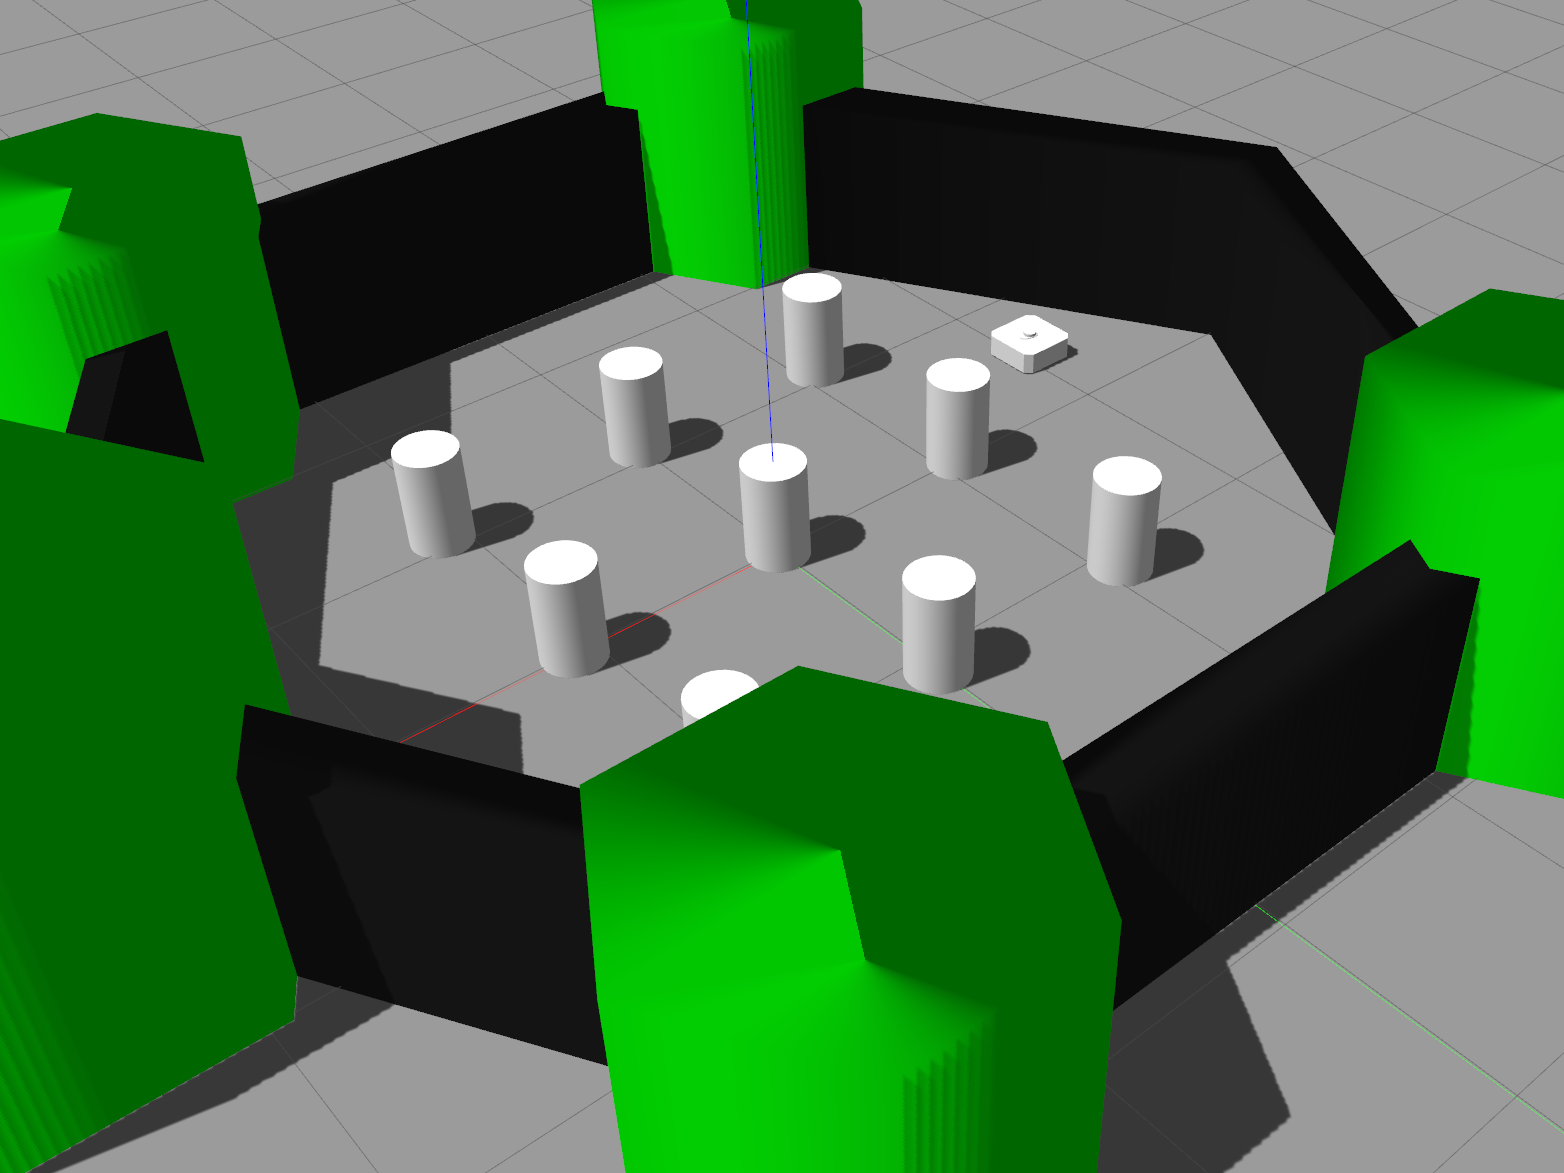
\includegraphics[width=0.75\textwidth]{images/world_env.png}
	\caption{Enclosed Environment in Gazebo}
	\label{fig:world_gazebo}
\end{figure}
\end{center}

The environments were mapped beforehand with the ROS2 "Slam Toolbox" package and provided via the Nav2 map server. 

The robot location and navigation goals are defined in another ROS Node, which programmatically spawns the robot into the environment and sets the goal this way. This way, the same scenario can be run with and without behavior planning. To test the behavior of the sensor failure fallbacks, the respective sensor driver, mentioned in chapter 4.5.1, was shut down to emulate the sensor's failure. 

\section{Scenarios}

The scenarios are derived from the functional requirements and can be used to test multiple requirements as listed in the tables \ref{tab:sensor_scenarios} and \ref{tab:behavior_scenarios}.
The acceptance criteria often contain multiple binary conditions that can only be met or failed. All acceptance criteria for a given scenario must be met for the test to be counted as a success.  

For the Lidar, IMU, and Odometry scenarios, the sensor driver was shut down when reaching the desired speed listed in the scenario. 
Scenario NoPathFound1 is a scenario in which the lifecycle state gets transitioned into "inactive" and can not execute the planning action anymore when triggered. The BT has to recover from the inability to plan in this scenario.
NoPathFound$\_$2 is simulating the scenario when the planner is active but fails to find a collision-free path to the desired goal. This scenario tests the ability to find alternative goals and navigate to a nearby goal. 
In the Collision$\_$1 scenario, an obstacle gets moved so close to the robot that a collision is registered. The forced collision tests the ability to escape a collision and resume navigation afterward. A new navigation goal is published after the behavior tree exits the Collision Fallback Routine.
Collision$\_$2 scenario is testing the same behavior but during active navigation. A flat obstacle is spawned in the path of the robot. The obstacle is too low to be detected by the laserscanner, and a collision occurs. The robot must be able to recover from the crash and keep on navigating towards the goal with an updated global path in this scenario. 
The Battery$\_$1 scenario tests if the robot tries to navigate toward a distant goal with a low battery charge. The simulated battery is emptied to a low level, and a new navigation goal is set. If the battery charge runs below zero percent during the navigation, the test fails. 

\begin{table}[ht]
	\caption{Sensor Scenarios}
	\label{tab:sensor_scenarios}
	\begin{tabular}{| m{0.1\textwidth} | m{0.17\textwidth}| m{0.3\textwidth} | m{0.3\textwidth}|} 
  	\hline
  	\textbf{Name} & \textbf{Related Requirements }& \textbf{Description} & \textbf{Success Criteria}\\ 
  	\hline
  	Lidar$\_$1 & fn$\_$req1, fn$\_$req2, fn$\_$req3, fn$\_$req4, fn$\_$req5 & Robot is standing still, Lidar node crashes & Reset the system\\ 
  	\hline
  	Lidar$\_$2 & fn$\_$req1, fn$\_$req2, fn$\_$req3, fn$\_$req4, fn$\_$req5 & Navigating with 0.25 m/s straight towards goal (1m away) & Reset system, reach goal \\ 
  	\hline
  	Lidar$\_$3 & fn$\_$req1, fn$\_$req2, fn$\_$req3, fn$\_$req4, fn$\_$req5 & Navigating with 0.25 m/s and 0.5 rad/s towards goal (1m away) & Reset system, reach goal\\
  	\hline
  	IMU$\_$1 & fn$\_$req1, fn$\_$req2, fn$\_$req3, fn$\_$req4, fn$\_$req5 & Robot is standing still, IMU node crashes & Reset system \\
  	\hline
  	IMU$\_$2 & fn$\_$req1, fn$\_$req2, fn$\_$req3, fn$\_$req4, fn$\_$req5 & Navigating with 0.25 m/s straight towards goal (1m away) & Reset system, reach goal \\ 
  	\hline
  	IMU$\_$3 & fn$\_$req1, fn$\_$req2, fn$\_$req3, fn$\_$req4, fn$\_$req5 & Navigating with 0.25 m/s and 0.5 rad/s towards goal (1m away) & Reset system, reach goal\\
  	\hline
  	Odom$\_$1 & fn$\_$req1, fn$\_$req2, fn$\_$req3, fn$\_$req4, fn$\_$req5 & Robot is standing still, Odom node crashes & Reset the system\\ 
  	\hline
  	Odom$\_$2 & fn$\_$req1, fn$\_$req2, fn$\_$req3, fn$\_$req4, fn$\_$req5 & Navigating with 0.25 m/s straight towards goal (1m away) & Reset system, reach goal \\ 
  	\hline
  	Odom$\_$3 & fn$\_$req1, fn$\_$req2, fn$\_$req3, fn$\_$req4, fn$\_$req5 & Navigating with 0.25 m/s and 0.5 rad/s towards goal (1m away) & Reset system, reach goal\\
  	\hline
 	\end{tabular}
\end{table} 	
  	
  	
\begin{table}[ht]
	\caption{Behavior Scenarios}
	\label{tab:behavior_scenarios}
	\begin{tabular}{| m{0.1\textwidth} | m{0.13\textwidth}| m{0.33\textwidth} | m{0.34\textwidth}|} 
	\hline
	\textbf{Name} & \textbf{Related Requirements} & \textbf{Description} & \textbf{Success Criteria}\\ 
  	\hline	
  	NoPath Found$\_$1 & fn$\_$req7 & Path to goal can not be calculated, robot is standing still &  
Reset system, calculate path to goal, reach goal \\
	\hline
	NoPath Found$\_$2 & fn$\_$req7, fn$\_$req8 & Goal is unreachable, robot is standing still & Alternative goals, close to the original are tested to be reachable \\
	\hline
	Collision$\_$1 & fn$\_$req2, fn$\_$req4, fn$\_$req6 & Robot is standing still and a collision with the robot is caused & Robot can get out of collision state, navigation to goals still working \\
	\hline
	Collision$\_$2 & fn$\_$req2, fn$\_$req4, fn$\_$req6 & The robot is driving and collides with an undetected obstacle (0.25m/s) &  
Robot can get out of collision state, navigation to goals still working, undetected obstacle gets added to map \\
	\hline
	Battery$\_$1 & fn$\_$req9 & The robot battery runs low & The robot will not drive to a goal that is outside of its reachable range \\
	\hline
	Motor$\_$1 & fn$\_$req2, fn$\_$req5 & Hardware failure on the motors & n.a. \\
	\hline
		
	\end{tabular}
\end{table}

\section{Results}

The results in table \ref{tab:results} show an increase in the successful handling of the test scenarios for most test cases. The system supervision component is very reliable and enables the system to recover from an unexpected sensor failure. The more advanced behaviors implemented can improve the autonomous handling of the scenarios. The Battery Scenario was successful every time it was induced. However, the path planning behavior for finding alternative goals was unsuccessful about 50 percent of the time. The test showed that alternative methods for finding new goals would probably have resulted in better performance. The collision behavior during driving worked well, and the map updates are an essential feature for the success of the scenarios.
Nevertheless, there is a lack of intelligence and autonomy when the robot stands still. A collision is forced, but the implemented behavior relies on the same mechanism as during the driving scenario. The missing differentiation led to a test case where the robot reversed into a wall because it was turned 90 degrees by the collision. That test failed because a human operator would be needed to correct the robot. This lack of robustness was not apparent in the driving collision scenario because the robot's force was insufficient to cause a significant shift in orientation when colliding with obstacles. 

\begin{table}[ht]

	\caption{Results}
	\label{tab:results}
	\begin{tabular}{| m{0.11\textwidth} | m{0.13\textwidth}| m{0.33\textwidth} | m{0.33\textwidth}|} 
  	\hline
  	\textbf{Name} & \textbf{Number of Runs} &  \textbf{Percentage Succesful Without Behavior Planning} & \textbf{Percentage Succesful With Behavior Planning}\\ 
  	\hline
  	Lidar$\_$1 & 5 & 0 & 100 \\ 
  	\hline
  	Lidar$\_$2 & 5 & 0 & 100 \\ 
  	\hline
  	Lidar$\_$3 & 5 & 0 & 100 \\ 
  	\hline
  	IMU$\_$1 & 5 & 0 & 100 \\ 
  	\hline
  	IMU$\_$2 & 5 & 0 & 100 \\ 
  	\hline
  	IMU$\_$3 & 5 & 0 & 100 \\ 
  	\hline
  	Odom$\_$1 & 5 & 0 & 100 \\ 
  	\hline
  	Odom$\_$2 & 5 & 0 & 100 \\ 
  	\hline
  	Odom$\_$3 & 5 & 0 & 100 \\ 
  	\hline
  	NoPath Found$\_$1 & 20 & 0 & 100 \\ 
  	\hline
  	NoPath Found$\_$2 & 20 & 0 & 55 \\ 
  	\hline
  	Collision$\_$1 & 20 & 0 & 95 \\ 
  	\hline
  	Collision$\_$2 & 20 & 0 & 100 \\ 
  	\hline
  	Battery$\_$1 & 10 & 0 & 100 \\ 
  	\hline
  	Motor$\_$1 & 10 & 0 & 0 \\ 
  	\hline
	\end{tabular}
\end{table} 

The architectural design choices meet all the non-functional requirements. 
Implementing the whole behavior planning and system supervision system eliminates a single point of failure for the system. Even when the Navigation2 system collapses, is the robot able to move to a degree and, more importantly, stop completely (compare table \ref{tab:tab:nonfn_req}, non$\_$fn$\_$req). The behavior tree and algorithms implemented in the behavior tree are all deterministic (non$\_$fn$\_$req3). The robots' behavior goes beyond pure reactivity when navigating through environments, as the advanced behaviors use a dedicated planning phase before the actions are carried out (non$\_$fn$\_$req4). 
Finally, the system's performance when checking the conditions of the BT is below the desired threshold of 10ms, as the whole system runs in multiple threads, which allows the behavior tree to complete one complete execution cycle in about 5ms with the current system. (non$\_$fn$\_$req2). 